\documentclass[11pt,a4paper,twoside,openright]{report}

\usepackage[top=25mm,bottom=25mm,right=25mm,left=30mm,head=12.5mm,foot=12.5mm]{geometry}
\let\openright=\cleardoublepage

\usepackage[a-2u]{pdfx}
\catcode30=12

\usepackage[
   backend=biber
%  ,style=iso-authoryear
  ,style=numeric
  ,citestyle=numeric
  ,sortlocale=cs_CZ
  ,bibencoding=UTF8
  %,block=ragged
]{biblatex}
\addbibresource{references.bib}

%% Přepneme na českou sazbu, fonty Latin Modern a kódování češtiny
\usepackage[czech]{babel}
\usepackage{lmodern}
\usepackage[T1]{fontenc}
\usepackage{textcomp}
\usepackage[utf8]{inputenc}

% Set fonts
\RequirePackage[osf]{mathpazo} % Palatino with oldstyle figures
\newcommand\liningnums[1]{\fontfamily{ppl}\selectfont#1}
\RequirePackage{eulervm}
\RequirePackage[scaled=.8819]{sourcecodepro} % Source Code Pro typeface for monospace

%%% Další užitečné balíčky (jsou součástí běžných distribucí LaTeXu)
\usepackage{amsmath}        % rozšíření pro sazbu matematiky
\usepackage{amsfonts}       % matematické fonty
\usepackage{amsthm}         % sazba vět, definic apod.
\usepackage{bm}             % tučné symboly (příkaz \bm)
\usepackage{graphicx}       % vkládání obrázků
\usepackage{fancyvrb}       % vylepšené prostředí pro strojové písmo
\usepackage{fancyhdr}       % prostředí pohodlnější nastavení hlavy a paty stránek
\usepackage{icomma}         % inteligetní čárka v matematickém módu
\usepackage{dcolumn}        % lepší zarovnání sloupců v tabulkách
\usepackage{booktabs}       % lepší vodorovné linky v tabulkách
\makeatletter
\@ifpackageloaded{xcolor}{
   \@ifpackagewith{xcolor}{usenames}{}{\PassOptionsToPackage{usenames}{xcolor}}
  }{\usepackage[usenames]{xcolor}} % barevná sazba
\makeatother
\usepackage{multicol}       % práce s více sloupci na stránce
\usepackage{caption}
\usepackage{enumitem}
\usepackage{lipsum}
\usepackage{wrapfig}
\setlist[itemize]{noitemsep, topsep=0pt, partopsep=0pt}
\setlist[enumerate]{noitemsep, topsep=0pt, partopsep=0pt}
\setlist[description]{noitemsep, topsep=0pt, partopsep=0pt}
\usepackage{pdfpages}

\usepackage{tocloft}
\setlength\cftparskip{0pt}
\setlength\cftbeforechapskip{1.5ex}
\setlength\cftfigindent{0pt}
\setlength\cfttabindent{0pt}
\setlength\cftbeforeloftitleskip{0pt}
\setlength\cftbeforelottitleskip{0pt}
\setlength\cftbeforetoctitleskip{0pt}
\renewcommand{\cftlottitlefont}{\Huge\bfseries}
\renewcommand{\cftloftitlefont}{\Huge\bfseries}
\renewcommand{\cfttoctitlefont}{\Huge\bfseries}

% vyznaceni odstavcu
\parindent=0pt
\parskip=11pt

% zakaz vdov a sirotku - jednoradkovych pocatku ci koncu odstavcu na prechodu mezi strankami
\clubpenalty=1000
\widowpenalty=1000
\displaywidowpenalty=1000

% nastaveni radkovani
\renewcommand{\baselinestretch}{1.20}

% nastavení hlavy a paty stránek
\fancyhf{}
\renewcommand{\chaptermark}[1]{\markboth{#1}{}}
\fancyhead[RO,LE]{\leftmark}
\fancyfoot[RO,LE]{\thepage}
%\renewcommand{\footrulewidth}{0pt}
\fancypagestyle{plain}{%
\fancyhf{} % clear all header and footer fields
\fancyfoot[RO,LE]{\thepage}
\renewcommand{\headrulewidth}{0pt}
%\renewcommand{\footrulewidth}{0.5pt}
}

% Tato makra přesvědčují mírně ošklivým trikem LaTeX, aby hlavičky kapitol
% sázel příčetněji a nevynechával nad nimi spoustu místa. Směle ignorujte.
\makeatletter
\def\@makechapterhead#1{
  {\parindent \z@ \raggedright 
   \Huge\bfseries \thechapter. #1
   \par\nobreak
   \vskip 20\p@
}}
\def\@makeschapterhead#1{
  {\parindent \z@ \raggedright 
   \Huge\bfseries #1
   \par\nobreak
   \vskip 20\p@
}}
\makeatother

% Trochu volnější nastavení dělení slov, než je default.
\lefthyphenmin=2
\righthyphenmin=2

% Zapne černé "slimáky" na koncích řádků, které přetekly, abychom si
% jich lépe všimli.
\overfullrule=1mm

%% Balíček hyperref, kterým jdou vyrábět klikací odkazy v PDF,
%% ale hlavně ho používáme k uložení metadat do PDF (včetně obsahu).
%% Většinu nastavítek přednastaví balíček pdfx.
\hypersetup{unicode}
\hypersetup{breaklinks=true}
\hypersetup{hidelinks}

%%% Prostředí pro sazbu kódu, případně vstupu/výstupu počítačových
%%% programů. (Vyžaduje balíček fancyvrb -- fancy verbatim.)

\DefineVerbatimEnvironment{code}{Verbatim}{fontsize=\small, frame=single}



\def\NazevPrace{Univerzální sériový programátor}
\def\Trida{R8.A}
\def\AutorPrace{Petr Šícho}
\def\DatumOdevzdani{25.3.2022}

% Vedoucí práce: Jméno a příjmení s~tituly
\def\Vedouci{Emil Miler}

% Studijní program a obor
\def\StudijniProgram{studijní program}
\def\StudijniObor{studijní obor}

% Text čestného prohlášení
\def\Prohlaseni{Prohlašuji, že jsem svou práci vypracoval samostatně a použil jsem pouze prameny a literaturu
uvedené v~seznamu bibliografických záznamů. Nemám žádné námitky proti zpřístupňování této práce v~souladu se
zákonem č. 121/2000 Sb. o~právu autorském, o~právech souvisejících s~právem autorským a
o~změně některých zákonů (autorský zákon) ve znění pozdějších předpisů.}

% Text poděkování
\def\Podekovani{%
Děkuji Emilovi Milerovi za pomoc při vedení této maturitní práce. Dále bych chtěl poděkovat open hardware komunitě, specificky pak Arduino komunitě, na jejíž fórem jsem našel značné množství informací.
}

% Abstrakt česky
\def\Abstrakt{%
Tato maturitní práce si klade za cíl zjednodušit proces programování a nahrávání do mikrokontrolérů v pozdře DIP. Univerzální sériový programátor (USP) je obvod, který je schopný, po vložení podporovaného čipu do ZIF patice, automaticky detekovat rozložení vývodů vloženého čipu. Na základě toho rozpozná o který model, či rodinu modelů, se jedná a uzpůsobí pro něj nahrávací obvod. Teoreticky by měl USP umět programovat všechny čipy pracující na 5 voltech a všechny dostatečně pomalé bit-banging protokoly, včetně těch, které vyžadují vysoké napětí (12V) pro resetování. 
}

% Abstrakt anglicky
\def\AbstraktEN{%
Abstract.
}

% 3 až 5 klíčových slov
\def\KlicovaSlova{programátor, čip, AVR, nahrávač, USP}
% 3 až 5 klíčových slov anglicky
\def\KlicovaSlovaEN{programmer, chip, AVR, uploader, USP}


\begin{document}

%%% Titulní strana práce a další povinné informační strany

%%% Titulní strana práce

\pagestyle{empty}
\pagenumbering{gobble}
\hypersetup{pageanchor=false}

\begin{center}
\LARGE
\textbf{GYMNASIUM JANA KEPLERA}\\
{\large Parléřova 2/118, 169 00 Praha 6}

\vspace{\stretch{3}}


\includegraphics[width=.3\textwidth]{img/logo}

\vspace{\stretch{3}}

{\Huge\bfseries\NazevPrace}

\vspace{8mm}
\mdseries{Maturitní práce}

\vspace{\stretch{8}}
\large
\begin{tabular}{rl}
Autor: & \AutorPrace \\
\noalign{\vspace{2mm}}
Třída: & \Trida\\
\noalign{\vspace{2mm}}
Školní rok: & 2021/2022\\
\noalign{\vspace{2mm}}
Předmět: & Informatika \\
\noalign{\vspace{2mm}}
Vedoucí práce: & \Vedouci \\
\end{tabular}

\vspace{20mm}
Praha, \DatumOdevzdani
\end{center}


\openright

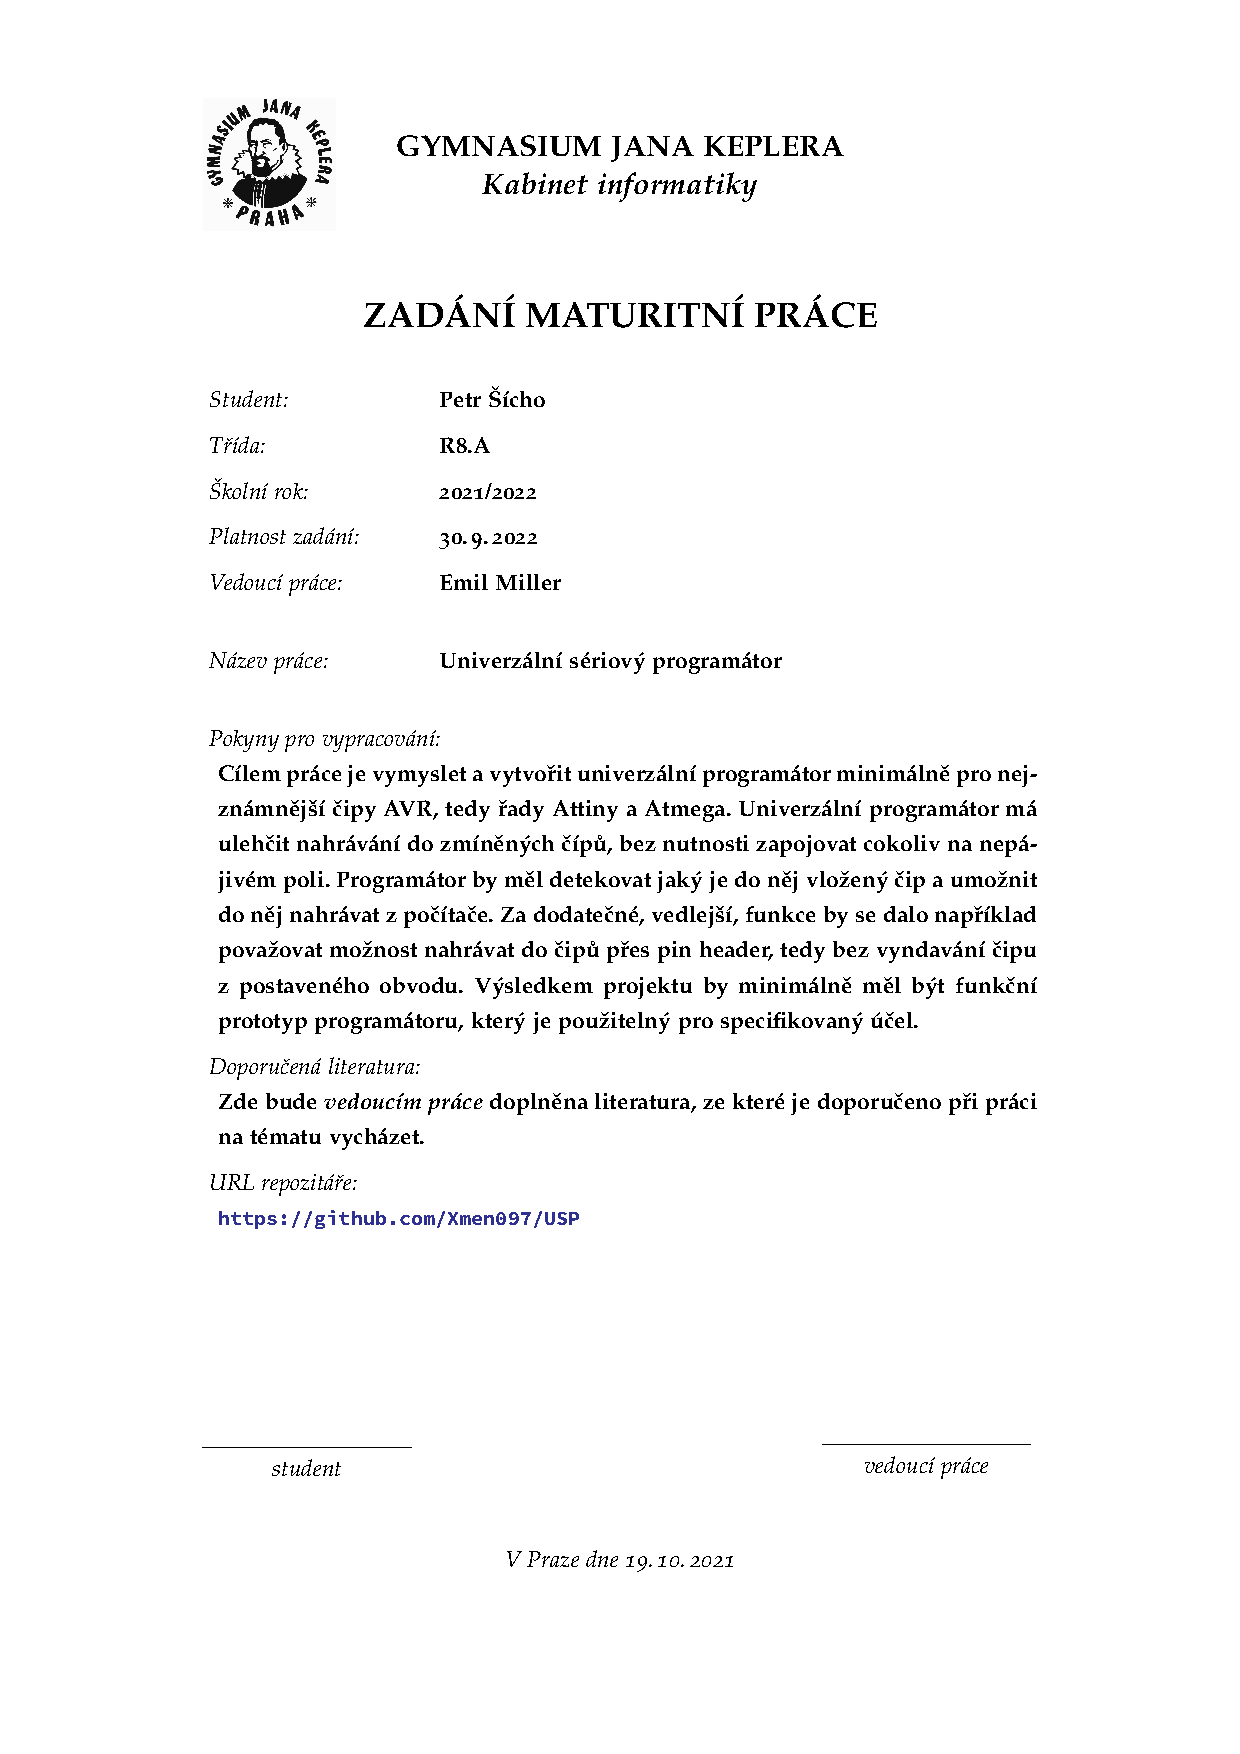
\includepdf[]{zadani.pdf}


%%% Strana s čestným prohlášením k bakalářské práci

\hypersetup{pageanchor=true}
\cleardoublepage
\vspace*{\fill}
\section*{Prohlášení}
\noindent
\Prohlaseni

\vspace{2cm}
\noindent
V Praze dne \today
\hspace*{\fill}\small{\AutorPrace}
\vspace{1cm}

%%% Poděkování
\openright
\vspace*{\fill}
\section*{Poděkování}
\noindent
\Podekovani
\vspace{1cm}


%%% Povinná informační strana bakalářské práce
\openright
\section*{Abstrakt}
\noindent
\Abstrakt
\subsection*{Klíčová slova}
\noindent
\KlicovaSlova

\vfill

\section*{Abstract}
\noindent
\AbstraktEN
\subsection*{Keywords}
\noindent
\KlicovaSlovaEN

\openright
\pagenumbering{arabic}

% Obsah
\setcounter{tocdepth}{2}
\tableofcontents

\chapter{Teoretická část}
\pagestyle{fancy}

Stejně jako existuje nepřeberné množství různých čipů, je také značné množství možných rozložení vývodů, které není jednotné ani u konkrétní velikosti. Pro každé rozložení je nutné mít nebo si postavit externí nahrávací obvod. Cílem USP je sjednotit tyto nahrávací obvody do jednoho univerzálního, který se přizpůsobí vloženému čipu. Programátor má tedy dvě principiální části - detekci a nahrávání. 

Chceme-li vytvořit opravdu univerzální programátor, není možné použít žádný dedikovaný hardware, který by zajišťoval nahrávání. Naopak se nám hodí použít univerzálních vstupních~/~výstupních pinů neboli GPIO pinů \footnote{z anglického General-purpose input/output, tedy pin, který se umí chovat buď jako digitální vstup, nebo výstup, přičemž mezi těmito módy je možné přepínat.}.

\section{Detekce}

Základem detekce je poznat jak velký čip je - tedy kolik má vývodů. Jen díky tomu se nám radikálně sníží počet možných kandidátů. Při zahrnutí jen několika modelů, jednoho pro každou velikost, bychom tak měli prakticky hotovo. Bylo by však nutné arbitrárně stanovit tyto podporované čipy, přičemž při vložení jiného, ať třeba ze stejné rodiny, který má prohozené piny GND a VCC, by došlo pravděpodobně k jeho zničení. Naší ambicí tedy bude zjistit o čipu co nejvíce informací, díky nimž budeme schopni rozeznávat mezi velkým počtem různých čipů.

Při všem musíme dbát, abychom čip nepoškodili. Budeme se snažit držet v hodnotách, které povoluje datasheet. Vzhledem k tomu, že to, o co se pokoušíme není standardní zacházení s čipy, nenalezneme v datasheetu konkrétní povolené hodnoty a situace, kterým můžeme čip bezpečně vystavit. Můžeme z něj ale vyčíst ale základní principy, kterých bychom se měli držet, abychom minimalizovali poškození čipu. Konkrétně se jedná o:
\begin{itemize}
	\item Nevystavovat žádný pin napětí nižšímu než $-0.5V$
	\item Nevystavovat žádný pin, kromě RESETu, napětí vyššímu než ${V}_{cc} + 0.5V$
	\item Nevystavovat RESET napětí vyššímu než $13V$
	\item Nenechat mezi žádný dvěma piny nezapojeného čipu téct nezanedbatelně velký proud po nezanedbatelně dlouhou dobu
\end{itemize}
Při splnění těchto podmínek by měl být čip dostatečně chráněn obvody, které běžně slouží k ochraně proti elektrostatickým výbojům (ESD), které jsou zabudovaná do prakticky všech čipů. \footnote{Pro naše účely budeme považovat za zanedbatelný proud řádu mikroampér a čas mikrosekund.}

\subsection {Detekce velikosti a polohy}

Detekce velikosti čipu nebude moc obtížná. Můžeme využít například toho, že každá reálná součástka, kromě svých primárních vlastností, vykazuje také elektrickou kapacitu. To bude jistě platit i pro spoje a součástky uvnitř integrovaných obvodů. Kapacita pinů jednoduchých CMOS\footnote{Complementary metal-oxide semiconductor; technologie výroby integrovaných obvodů} se pohybuje řádově v hodnotách pikofaradů\. Není mi znám žádný způsob přímého měření elektrické kapacity, budeme tedy muset provést měření nepřímé. Využijeme rovnici definující elektrický kondenzátor







\chapter{Implementace}

Druhá kapitola obsahuje detailní informace o tom, jak probíhala implementace. Zde se objeví zdůvodnění výběru technologií, řešení problémů, na které jste narazili, informace o použitých knihovnách apod. Pochvalte se, nikdo to za Vás neudělá. Přiznejte chyby, není to ostuda.

\section{Ukázka sekce}

\lipsum

\chapter{Technická dokumentace}

Poslední kapitola obsahuje informace o tom, jak projekt, který v rámci maturitní práce vznikl, nainstalovat, spustit a používat.

\section{Ukázka sekce}

\lipsum[5]

\subsection{A jedné podsekce}

\lipsum

\section{A další sekce}

\lipsum

\chapter*{Závěr}
\pagestyle{empty}
\addcontentsline{toc}{chapter}{Závěr}

Závěr obsahuje shrnutí práce a vyjadřuje se k míře splnění jejího zadání. Dále by se zde mělo objevit sebehodnocení studenta a informace o tom, co nového se naučil a jak vnímal svou práci na projektu. \cite{einstein}

%%% Seznam použité literatury
\nocite{einstein}\nocite{latexcompanion}\nocite{knuthwebsite}
\printbibliography[title={Seznam použité literatury},heading={bibintoc}]

%%% Seznam obrázků
\openright
\listoffigures
\addcontentsline{toc}{chapter}{Seznam obrázků}

%%% Seznam tabulek
\clearpage
\listoftables
\addcontentsline{toc}{chapter}{Seznam tabulek}

%%% Přílohy k práci, existují-li. Každá příloha musí být alespoň jednou
%%% odkazována z vlastního textu práce. Přílohy se číslují.

%\part*{Přílohy}
%\appendix

\end{document}
